\cotefile{80}
\scanpage{39}
% slanted
\margin{\unsure{correspondent|corresp.|correspond.} $\longrightarrow$\\ à \deleted{\unsure{$\mathfrak S_4\times\{\pm1\}$}}\\ $\unsure{\widetilde{\mathfrak S}_{4}|\widetilde{\mathscr S}_{4}|\widetilde{S}_{4}|\mathfrak S_4}\longrightarrow\mathfrak S_4\times\{\pm1\}\longrightarrow\widetilde{\mathfrak S}_4$}%
où les flèches marquées $\approx$ sont des équivalences,
les flèches marquées $\mathrel{\tikz[baseline=-.45ex]{\draw[->] (0,0)--(.84,0); \draw[dotted] (.08,.02) to[bend left=100] (.12,.15);}}$ sont fidèles, la
flèche $\mathrel{\tikz[baseline=-.45ex]{\draw[->] (0,0)--(.84,0); \draw[dotted] (.81,.02) to[bend right=105] (.66,.17);}}$ est \deleted{\unsure{de}}surjective sur les ens. d'homomorphismes,
la flèche \deleted{verticale} $\mathrel{\tikz[baseline=-.45ex]{\draw[->] (0,.21)--(0,-.21); \node[left,inner sep=.7pt] at (0,.06) {\scriptsize 1};}}$ est \deleted{de}
identité de (oct. g.). La face supérieure du
cube est formée des objets ``orientés'', les quatre
flèches constituant ce carré sont des équivalences ;
la face inférieure est \deleted{\unsure{formée}}\inserted{formée} des objets
non orientés, \deleted{\unsure{dont les sont}} les deux flèches
$\textrm{oct}\longrightarrow\textrm{gr. oct.}\longrightarrow\textrm{gr. oct g.}$ sont des équivalences,
les deux autres sont resp. surjectives sur \inserted{les} hom,
et fidèles. Les quatre flèches de passage
de la théorie orientée vers la non orientée sont
fidèles. La face de gauche est formée des
objets ``ordinaires'' \deleted{ou} ``sphériques'', celle de
droite est formée des objets ``gauches'' ou
``projectifs'', les \inserted{quatre} flèches de passage de l'une
à l'autre sont des équivalences, à l'exception
de $\textrm{oct}\longrightarrow\textrm{oct. gauche}$ (surjectif sur les
hom). La face postérieure du cube est
formée des configurations deux-dimensionnelles,
\deleted{celle} la face antérieure est formée des
configurations $1$-dimensionnelles associées, les
quatre flèches de passage sont des équivalences
sauf $\textrm{oct. g}\longrightarrow\textrm{gr. oct. gauche}$, qui est fidèle
et fait l'objet de l'énoncé (16) plus haut.
% archive sheet number: 38

\scanpage{40}\mspage{5}
% archive sheet number: 39
On appellera \uline{orientation} de $(K,(D_i)_{i\in J})$, la
donnée, pour $\forall\, I\in\unsure{\mathfrak P_3|\mathcal P_3}(J)$ comme dessus
(de $\forall$ ens. de 3 pseudo-droites non concourantes),
d'une \uline{orientation} \inserted{$\omega_I$} du graphe
octaédral gauche correspondant.

Soit maintenant $\mathcal X$ une \uline{carte} qui
soit un arrangement de pseudo-droites.
Son 1-squelette \inserted{$K$} est alors muni de \deleted{une}\inserted{\unsure{$\mathcal C$|la}}
famille $(D_i)_{i\in J}$ de pseudo-droites, c'est
donc un arrangement $\underline{1}$ dim. de
ps. droites. De plus il est muni d'
une orientation naturelle $\omega=(\omega_I)_{\substack{I\in\mathfrak P_3(J)\\\bigcap_{i\in I}D_i=\varnothing}}$.

On trouve ainsi un foncteur
\[\mathcal X\longmapsto (K,(D_i)_{i\in J},\omega)\tag*{(18)}\]
de \unsure{lá|la} catégorie des arrangem\textsuperscript{ts} comb. de
pseudo-droites, vers la catégorie combinatoire
des arrangem\textsuperscript{ts} $1$ dimensionnels orientés de
pseudo-droites.

% slanted
\margin{\deleted{\unsure{Il faut restreindre} le foncteur aux} Il est vrai que \unsure{si l'on} se limite aux \unsure{composantes|comp.} \unsure{comp. part.} qui ne \unsure{corr. pas} \unsure{de} \unsure{trigones|trigones et} \unsure{bigônes|bigones|bigone}}%
\uline{\unsure{Prop\textsuperscript{n}.|Prop.|Th.}} Le foncteur précédent est \uline{pleinement}
\uline{fidèle}, i.e. pour deux arrangem\textsuperscript{ts} comb.
$\mathcal X,\mathcal X'$ de ps. droites, on a
\[\operatorname{Isom}(\mathcal X,\mathcal X')\xrightarrow{\sim}\operatorname{Isom}\big((K,(D_i)_{i\in J},\omega),(K',(D'_{i'})_{i'\in J'},\omega')\big)\]

\scanpage{41}
Soit $K$ un 1-complexe\unsure{s|{}} combinatoire fini,
$(D_i)_{i\in J}$ \deleted{une} \deleted{\unsure{$f$}} ens. fini de sous-complexes
polygonaux, tels que toute arête de $K$ appartienne
à un $D_i$ et un seul, \deleted{et que $K$ n'ait pas
de sommet isolé i.e. $\forall$ sommet de $K$
appartient à au moins un des $D_i$.} On
suppose de plus que \deleted{si} $i\ne j$, $D_i$ et $D_j$
ont en commun un sommet et un
seul, et que $\forall$ sommet \inserted{de $K$} appartient à au
moins 2 des $D_i$. On dit alors que
$(K,(D_i)_{i\in J})$ est un arrangement \inserted{\deleted{\unsure{linéaire}}1-dimensionnel} de ps. droites,
\deleted{\unsure{$\forall$}} pourvu que l'intersection des $D_i$ soit vide.
i.e. que $K$ ne soit pas simplement le ``\unsure{point|joint}''
d'une famille de \deleted{polygones}\inserted{monogones (ou ``boucles'')}
rattachés par un sommet \inserted{\unsure{en|un}} commun. Il existe alors
tjrs au moins une partie $I\subset J$ de cardinal
3, tel que les $D_i$ $(i\in I)$ n'aient
pas de pt en commun. \deleted{$D_i$, \unsure{le}} \inserted{Pour}
% slanted
\margin{\uline{NB} L'ordre \unsure{$\nu_i$|ici} des polygônes $D_i$ \unsure{cf.} est \unsure{donc} \unsure{tjrs|tjs} $\geq 2$, pour un arrangem\textsuperscript{t} : aucun des $D_i$ n'est un monogône\ldots}%
\deleted{Pour} \unsure{tt|une} partie $I$ de $J$, soit $K_I$ le ss-complexe
de $K$ \inserted{qui ``topologiquement'' est} réunion des $D_i$ $(i\in I)$
% slanted
\margin{\uline{NB} $K_I$ sera regardé comme arrangem\textsuperscript{t} 1-dim de ps. droites, grâce aux $D_i$ $(i\in I)$, OK. si les $D_i$ ne sont pas \deleted{\unsure{con}} concourantes (il faut donc $\operatorname{card} I\geq 3$)}%
\inserted{mais où on prend comme sommets que les intersections des $D_i$ deux à deux.}
Dans le cas qui nous intéresse $(\operatorname{card} I=3,
\bigcap_{i\in I}D_i=\varnothing)$ \deleted{\unsure{on}} $K_I$ est un graphe
octogonal gauche, donc on peut parler
d'\uline{orientation} de ce graphe octogonal g.
% archive sheet number: 40

\scanpage{42}\mspage{6}
Pour le voir, on va montrer comment la
carte $\mathcal X$ peut être reconstruite à partir de
l'arrangement 1-dimensionnel orienté. Par la
théorie générale des cartes, il revient au même,
\deleted{\unsure{de}} comme les sommets de $K$ sont d'ordre
$\geq4$ (\deleted{\unsure{$\geq$}}à fortiori $\geq3$), de construire, à partir
de $(K,(D_i)_{i\in I},\omega)$, :

1\textsuperscript{o}) Pour \deleted{tout} $s\in S$ (ens. des sommets de $K$) \deleted{\unsure{le}}
l'ens. \[\inserted{\vec{\unsure{Z|\mathcal Z|\mathfrak Z}}_s\unsure{\in|\subset}\deleted{A}{\unsure{\mathfrak S|\mathscr S|\mathcal C}}_{\vec A_s}}\tag*{(19)}\] des deux ordres circulaires \inserted{(inverses l'un de l'autre)}
canoniques sur l'ens. \inserted{$\vec A_s$} des \deleted{arêtes}\inserted{arcs} de $K$ d'origine
$s$, qu'on peut identifier \deleted{au} \unsure{sic|à} : l'ens
$\vec I_s$ des ps. droites \uline{orientées} \inserted{$\vec D_i$} passant par $s$.

2\textsuperscript{o}) Pour \deleted{\unsure{deux sommets $s,s'$|toute arête orientée}} \deleted{tout} arc $\vec a\in\vec A$ de $K$, d'origine
$s$ et d'extrémité $s'$, la bijection canonique
\[\psi_{\vec a}:\vec Z_s\xrightarrow{\sim}\vec Z_{s'}\tag*{(20)}\]
(qui donne lieu à \unsure{la|l'} \deleted{\unsure{ég}}formule
\[\psi_{-\vec a}=(\psi_{\vec a})^{-1}\tag*{(21)}\]

Quand je dis ``canonique'', j'entends :
provenant de la donnée de la carte $\mathcal X$.
Inversement, si on a pu, à partir de $(K,(D_i)_{i\in I},\omega)$,
construire intrinsèqu\textsuperscript{t} des données
(19) et (20) satisfaisant (21), on trouve une
immersion cellulaire combinatoire de
$K$ dans un $\mathcal X$ (peut être pas le plan projectif !).
% archive sheet number: 41

\scanpage{43}
Pour savoir que $(D_i)_{i\in J}$ y forme bien un
système de ps. droites, il faudra d'abord voir
qu'ils se \unsure{déduisent|relèvent} de la structure de carte
de la façon habituelle, ce qui s'exprime
par la condition (où $s\in S$)
\[\left\{\begin{aligned}
&\text{Si }\rho\in\vec{\unsure{Z|\mathcal Z|\mathfrak Z}}_s,\ \deleted{\unsure{de}}\ \text{et si }{\nu}_s\text{ est le nb de }D_i\text{ passant}\\
&\text{par }s,\ \text{on a }\rho^{\nu_s}(\vec D_i)=(-\vec D_i)\quad\text{pour }\unsure{\text{tte}|\forall}\\
&\text{droite orientée }\inserted{\vec D_i}\text{ passant par }s.
\end{aligned}\right.\tag*{(22)}\]
% slanted
\margin{\uline{NB} Si $\nu_s=2$, alors la condition (22) implique déjà la connaissance de $Z_s\subset{\unsure{\mathfrak S|\mathscr S|\mathcal C}}_{\unsure{\vec D_s|\vec A_s|\vec I_s}}$.}

\deleted{En d'autres termes,}
% slanted
\margin{\uline{\unsure{plus|selon}} la \uline{connexité} de $\mathcal X$ i.e. celle de $K$.}
Il faudra de plus que $\mathcal X$ soit le plan projectif,
ce qui s'exprime par la condition d'EP
\[\underbrace{c_0-c_1}_{1-c(K)}+c_2=1\qquad\text{soit}\quad c_2\deleted{\unsure{(K)}}=c(K)\tag*{(23)}\]
\inserted{\deleted{\unsure{connexité}} degré de connexion de $K$}
% slanted
\margin{\uline{NB} On aura a priori $c_2\leq c(K)$, la formule (23) exprime que la borne sup. est atteinte\ldots}
$c_0=\operatorname{card} S$, $c_1=\operatorname{card} A$ (nb de sommets et
nb d'arêtes) ne dépendent que $K$, tandis que
$c_2$ \inserted{(nb de faces)} dépend bien sûr de $\mathcal X$.

\uline{Construction des} $\vec Z_s$ satisfaisant (22). On
va d'abord définir, pour $\nu_s\geq3$
\[Z_s^{\unsure{\prime|1}}\subset\mathfrak S_{I_s}\tag*{(24)}\]
\unsure{ensem.|comme ens.} de deux ordres circulaires opposés
l'un à l'autre, sur l'ens \inserted{$I_s$} des ps droites passant
% slanted
\margin{i.e. une structure \uline{polygonale} sur cet ens.}
par $s$. Soit $\Delta$ \deleted{$D$} une ps. droite qui ne
passe pas par $s$. \deleted{Alors ch\textsuperscript{une} des ps. droites \inserted{$D_i$}
passant par $s$ est en corr. biunivoque avec l'} \inserted{\unsure{Cons.}, \deleted{\unsure{une $D_s$}} application}
% archive sheet number: 42

\scanpage{44}\mspage{7}
canonique
\[\begin{aligned}
I_s\ \deleted{\unsure{D_i}}&\mathrel{\mathop{\longmapsto}\limits^{\varphi=\varphi_{s,\Delta}}}\deleted{\unsure{D_i\cap\Delta}}\ \text{ens. }\deleted{\text{des}}\ S_\Delta\text{ des sommets}\\
&\hspace{3em}\text{de }K\text{ sur }\Delta
\end{aligned}\tag*{(25)}\]
caractérisée par
\[\deleted{\unsure{\text{ou}}}\qquad D_i\cap\Delta=\{\varphi(\unsure{D|i|D_i})\}\]
Cette application est \uline{injective}, \deleted{et} i.e.
\[\varphi_{s,\Delta}:I_s\lhook\joinrel\longrightarrow S_\Delta\]
Comme sur $S_\Delta$ (ens des sommets d'un polygône)
il y a une structure polygônale, il y a sur
$I_s$ une structure polygonale induite, \deleted{\unsure{donc}}
soit $\deleted{\unsure{\varphi|Z}}Z_{s,\Delta}^{\unsure{\prime|1}}$. On aura alors

% slanted
\margin{Condition en les sommets $s$ tels que $\nu_s\geq3$.}
\[\begin{aligned} &Z'_{s,\Delta}\text{ est indépendant du choix de}\\
&\Delta\in I\setminus I_s,\quad\text{soit } Z'_s.
\end{aligned}\tag*{(A1)}\]
% slanted
\margin{à prouver que c'est vrai quand on part d'un $\mathcal X$ (et qu'on trouve bien le $Z_s$ \uline{déduit} de $Z_s$\ldots) \unsure{itou|idem|item} pour la variante avec $\vec\Delta$, \unsure{plus fine|plus loin}.}
\deleted{On} Considérons l'application
\[\vec I_s\longrightarrow I_s\qquad\text{de degré }2\tag*{(26)}\]
\deleted{On doit}\inserted{On aura} alors
\[\left\{\begin{aligned}
&\text{si }\deleted{\unsure{\rho|\varphi}}\,\vec u\in\vec{\unsure{Z|\mathcal Z|\mathfrak Z}}_s\inserted{\in{\unsure{\mathfrak S|\mathscr S|\mathcal C}}_{\vec I_s}},\quad\vec u\text{ passe au quotient dans (26),}\\
&\text{en }u\deleted{\unsure{'} }\in\mathfrak S_{I_s},\quad\text{et on a }u\in Z'_s.
\end{aligned}\right.\tag*{(27)}\]
C'est là une condition restrictive importante
sur la structure polygônale $\vec Z_s$ qu'on veut déterminer,
qui limite le choix à $2^{\nu_s-1}$ possibilités,
% archive sheet number: 43

\scanpage{45}
comme on voit ainsi. \deleted{On fixe $u_0\in Z'_s$,
et une origine $i_0\in I_s$, d'où $i_1\ldots i_{\nu_s-1}$ donnés
par}
\[\deleted{i_\nu=u_0^{\nu}i_0}\]
\deleted{Soit $\omega_\nu$ l'une des deux orientations de $D_{i_\nu}$ i.e. la
\deleted{\unsure{un de|l'un}} fibre de $i_\nu$ dans (26), alors $u$
est connue}

On fixe $u_0\in Z_s^{\unsure{\prime|1}}$, i.e. une
orientation du polygone d'ens de
sommets $I_s$, pour chaque
$i\in I_s$, on doit se donner une
bijection \inserted{$\alpha_i$} de $\unsure{\vec I_i|\vec I_{2i}}$ la fibre de
$\vec I_s$ en $i$, \{i.e. de l'ens \inserted{$\omega_i$} des
deux orientations de $D_i$\}
\figure{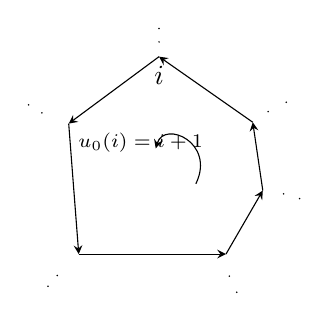
\begin{tikzpicture}[scale=.85,>=stealth]
\coordinate (t) at (0,2.0); \coordinate (l) at (-1.35,1.0);
\coordinate (bl) at (-1.2,-.95); \coordinate (br) at (1.0,-.95);
\coordinate (r) at (1.55,0); \coordinate (tr) at (1.4,1.02);
\draw[->] (t)--(l); \draw[->] (l)--(bl); \draw[->] (bl)--(br);
\draw[->] (br)--(r); \draw[->] (r)--(tr); \draw[->] (tr)--(t);
\draw[->] (.55,.1) .. controls (.85,.72) and (.08,1.05) .. (-.05,.63);
\node[below] at (t) {$i$}; \node[below right,font=\scriptsize] at (l) {$u_0(i)=i+1$};
\foreach \x/\y in {0/2.22,0/2.42,-1.75/1.16,-1.95/1.28,-1.52/-1.27,-1.66/-1.43,1.05/-1.28,1.16/-1.52,1.86/-.05,2.1/-.12,1.63/1.18,1.9/1.32}{\fill (\x,\y) circle (.013);}
\end{tikzpicture}}
avec $\omega_j$ où $j=u_0(i)$ est le sommet suivant $i$
— ce qui, pour $i$ fixé, fait 2 choix, donc
en tout, en apparence, $2^{\nu_s}$ choix. Mais on
veut que la permutation $u$ de $\vec I_s$ obtenue
soit une permutation circulaire, i.e. \deleted{soit}
transitive ; si on fixe $i_0\in I$ \inserted{et on pose $i_{\unsure{\alpha|\nu}}=u_0^{\unsure{\nu|\alpha}}(i_0)$}
cela signifie que
les choix de $\alpha_{i_0},\alpha_{i_1},\ldots,\alpha_{i_{\nu_s-2}}$
\margin{$\nu=\nu_s$}
\[\omega_{i_0}\mathrel{\mathop{\rule{1.8em}{.4pt}}\limits^{\substack{\alpha_{i_0}\\\sim}}}\omega_{i_1}
\mathrel{\mathop{\longrightarrow}\limits^{\substack{\alpha_{i_1}\\\sim}}}\omega_{i_2}\quad\ldots\quad
\omega_{i_{\nu_s-2}}\mathrel{\mathop{\longrightarrow}\limits^{\substack{\alpha_{i_{\nu_s-2}}\\\sim}}}\omega_{i_{\nu_s-1}}\tag*{(28)}\]
déterminent le choix du dernier $\alpha_{i_{\nu-1}}:\omega_{i_{\nu-1}}\mathrel{\mathop{\rule{1.6em}{.4pt}}\limits^{\sim}}\omega_{i_\nu}=\omega_{i_0}$
par la condition qu'il soit \uline{distinct} \inserted{(i.e. que ce soit l'\uline{opposé})} \deleted{du composé}
l'inverse du composé des bij. précédentes.
\deleted{Dans le cas où}
% archive sheet number: 44

\scanpage{46}\mspage{8}
Soit $\vec\Delta$ une \inserted{ps-}droite \uline{orientée} ne passant pas
par $s$, alors l'orientation de $\vec\Delta$ en \unsure{définis|définit} une
de $I_s\subset S_\Delta$, i.e. un générateur $u_0$, noté
$(u_{\deleted{\unsure{\Delta}}s,\vec\Delta}$, de $Z_s^{\unsure{\prime|1}}=Z'_{s,\Delta}$. Si $\unsure{\nu_2|v_2|\nu_s}=2$, on prendra
$u_{s,\vec\Delta}$ la transposition de $I_s$ (de card 2), égal
ici à son inverse (i.e. \deleted{\unsure{$Z_s$}} ici $\operatorname{card} Z'_s=1$, et non 2).

On \deleted{doit} \deleted{doit} définir un $\vec u_{s,\vec\Delta}$ au dessus de
\deleted{\unsure{$u_s$}} $u_{s,\vec\Delta}$, ce qui fait (en exigeant que
soit une permutation circulaire) \inserted{un choix à déterminer parmi} $2^{\nu_s-1}$ \deleted{\unsure{de}}
possibilités \inserted{a priori}. (Le compte est bon, même pour
$\nu_s=2$). On est ramené ici, pour une ps-droite
$D_i$ passant par $s$, désignant par
$D_j$ son ``successeur'' pour $u_{s,\vec\Delta}$, à décrire
la bijection $\omega_i\xrightarrow{\sim}\omega_j$ induite par $\vec\Delta$,
donc pour le choix d'une
orientation sur \inserted{$D={}$} $D_i$, d'où
$\vec D_i$, il faut décrire
l'orientation correspondante de $D_j$ — en utilisant
l'orientation de $\vec\Delta$.

\figure{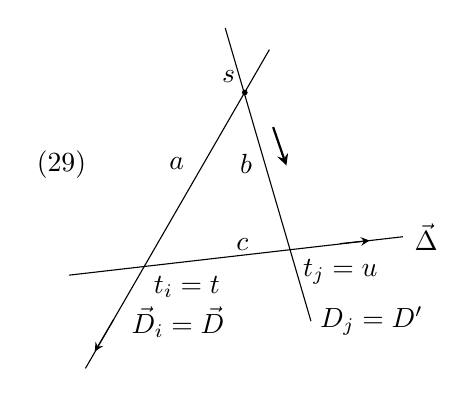
\begin{tikzpicture}[scale=.80,>=stealth]
\draw (-1.92,-2.40)--(1.00,2.66);
\draw (.30,3.00)--(1.66,-1.65);
\draw (-2.18,-.92)--(3.12,-.31);
\fill (.61,1.98) circle (.045) node[above left] {$s$};
\draw[->] (-1.47,-1.62)--(-1.77,-2.13);
\draw[->,thick] (1.06,1.43)--(1.27,.82);
\draw[->] (2.12,-.42)--(2.59,-.37);
\node at (-.47,.85) {$a$}; \node at (.63,.84) {$b$}; \node at (.57,-.44) {$c$};
\node[below right] at (-.99,-.78) {$t_i=t$}; \node[below right] at (1.38,-.51) {$t_j=u$};
\node at (-.45,-1.67) {$\vec D_i=\vec D$}; \node[right] at (1.65,-1.65) {$D_j=D'$};
\node[right] at (3.15,-.31) {$\vec\Delta$}; \node at (-2.30,.83) {(29)};
\end{tikzpicture}}
La figure montre que l'orientation à choisir sur
$D'=D_j$ est décrite par la condition que l'arête \inserted{$a$} \uline{joignant}
$s$ à $t=\varphi(i)$ (intersection de $D$ et $\deleted{\unsure{\leftarrow|\rightarrow}}\Delta$), dans le sens
de l'orientation \deleted{\unsure{donnée}} de $\vec D$, et celle $b$ joignant $s$ à $u=\varphi(j)$
(int. de $D'$ et $\Delta$) dans le sens de l'orientation cherchée de
$D'$, et enfin l'arête $c$ joignant $t$ à $u$ dans le sens
% archive sheet number: 45

\scanpage{47}
de) l'orientation de $\vec\Delta$, soit un syst. \deleted{\unsure{for}}
d'arêtes \uline{appartenant à l'orientation} du \deleted{triangle}
% slanted
\margin{i.e. (\unsure{intuitivement|orientations}) qu'ils bordent un $=$ triangle\ldots}
$\omega_{\{i,j,\Delta\}}$ de l'arrangem\textsuperscript{t} des trois ps. droites
$\Delta,D,D'$ (ce qui caractérise l'orientation de
$\vec D'$, parmi les deux de $D'$, en termes de
celles de $\Delta,D$).

(A2) Cette prescription — qui définit, \deleted{\unsure{une}} pour
$s,\vec\Delta$ fixés, une permutation $\vec u_{s,\vec\Delta}$ de $\vec I_s$
au dessus de la permutation $u_{s,\vec\Delta}$ de $I_s$)
est bien une permutation \uline{circulaire}
\deleted{\unsure{involution sans être}} i.e. $(\vec u_{s,\vec\Delta})^{\unsure{\nu_s|v_s}}$ (qui est, \deleted{soit}
a priori, soit l'identité, soit l'\deleted{autre} transposition
sur chaque fibre de (26)) \deleted{n'est} est la transposition.

\deleted{(A3) Si $\vec{\Delta'}$ est \unsure{$\to$}}
\uline{NB} On aura \deleted{\unsure{$\vec u$}}
\[\begin{aligned}\vec u_{s,-\vec\Delta}&=\vec u_{s,\vec\Delta}^{-1},\qquad\text{posons}\\
\vec{\unsure{Z|\mathcal Z|\mathfrak Z}}_{s,\Delta}&=\{\vec u_{s,\vec\Delta},\vec u_{s,-\vec\Delta}\}\subset{\unsure{\mathfrak S|\mathscr S|\mathcal C}}_{\vec I_s}
\end{aligned}\tag*{(30)}\]

(A3) Soit $\Delta'$ une autre ps-droite ne passant pas
par $s$, alors on a
\[\vec Z_{s,\Delta'}=\vec Z_{s,\Delta}\qquad(\text{soit }\vec Z_s)\]

Bien entendu, les conditions (A1) à (A3)
sont satisfaites pour un arrangem\textsuperscript{t} \inserted{1-dim.} orienté
de ps. droites \uline{provenant} d'un arrangem\textsuperscript{t} 2-dimensionnel,
ce que permet donc de
% archive sheet number: 46

\scanpage{48}\mspage{9}
construire les $\vec{\unsure{Z|\mathcal Z|\mathfrak Z}}_{s,\deleted{\unsure{\Delta}}}$ \inserted{$(s\in S)$}, et l'application
surjective
\[\vec I_{\deleted{\unsure{s}}}\setminus\vec I_s\longrightarrow\vec Z_{\unsure{s,|s;|s}}\tag*{(31)}\]
de l'ens des \unsure{pseudo-dr.|ps. dr.} orientées ne passant pas
par $s$, dans $\vec Z_s$, application compatible avec
l'action du groupe des signes $\pm1$.

Soit maintenant $\vec a$ un arc de
$K$, joignant $s$ à $s'$, on veut définir
\[\psi_{\vec a}:\vec Z_s\longrightarrow\vec Z_{s'}\]
\deleted{C'est ici qu'on a besoin de} \inserted{Supposons d'abord} l'existence
d'au moins une ps-droite qui ne passe
pas par $s$ ni $s'$. Considérons
\diagram{\begin{tikzcd}[ampersand replacement=\&,column sep=.9em,row sep=1.7em]
\& \& {\vec J=\vec I\setminus(\vec I_s\cup\vec I_{s'})}\arrow[dl]\arrow[dr] \& \\
{(32)} \& \vec Z_s\arrow[rr,dashed,"\psi_{\vec a}"] \& \& \vec Z_{s'}
\end{tikzcd}}
on obtient deux quotients de $\vec J$ — on
devra faire condition que c'est le $\overline{\textrm m}$, i.e.

(A4) si $\vec\Delta,\vec{\Delta'}$ sont deux ps. droites orientées
ne passant pas par les extrémités $s,s'$ de
l'arête $a$, qui induisent la $\overline{\textrm m}$ orientation en
$s$, elles induisent aussi la $\overline{\textrm m}$ orientation en $s'$.
% archive sheet number: 47

\scanpage{49}
Reste à traiter le cas (très particulier !) où
$\nexists$ ps. droite $\Delta$ qui ne passe par $s$ ni par $s'$.
\inserted{Soit $\Theta$ la ps. droite déterminée par $a$,}
Considérons alors une ps. droite $D$ \inserted{$\ne\Theta$} passant par
$s$, \deleted{\unsure{soit}} une $D'$ \inserted{$\ne\Theta$} passant par $s'$,
\deleted{\unsure{on|soit}} a donc $D\ne D'$, soit
$t$ l'intersection de $D$ et $D'$.
Soit, \deleted{\unsure{$b$ une des deux|$b$ une des|$b$ un des deux}} \inserted{$K'={}$} $K_{\{\Theta,D,D'\}}$,
\figure{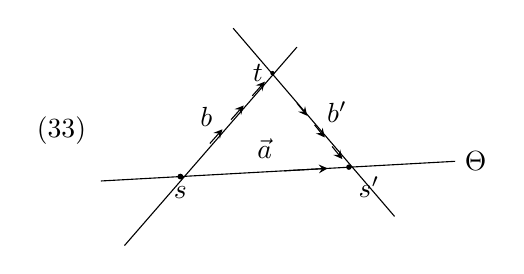
\begin{tikzpicture}[>=stealth]
\draw (-2.15,-.12)--(2.35,.13) node[right] {$\Theta$};
\draw (-1.85,-.94)--(.34,1.58); \draw (-.47,1.82)--(1.58,-.57);
\coordinate (s) at (-1.14,-.064); \coordinate (t) at (.03,1.25); \coordinate (h) at (1.0,.056);
\fill (s) circle (.037) node[below] {$s$}; \fill (t) circle (.028) node[left] {$t$}; \fill (h) circle (.035) node[below right] {$s'$};
\foreach \p in {.32,.55,.78}{\draw[->] ({-1.14+1.17*\p},{-.064+1.314*\p})--++(.16,.18);
\draw[->] ({.03+.97*\p},{1.25-1.194*\p})--++(.13,-.16);}
\draw[->] (.18,.009)--(.73,.04); \node[above] at (-.07,.04) {$\vec a$}; \node[left] at (-.61,.70) {$b$}; \node[right] at (.60,.75) {$b'$}; \node at (-2.65,.52) {(33)};
\end{tikzpicture}}
$b$ une des arêtes qui joignent $s$ à $t$, et prenons
l'unique arête $b'$ de $\unsure{\widetilde K'|K'}$ qui joigne $t$ à $s'$, et
telle que $\{a,b,b'\}$ soit compatible avec l'
orientation de $K'$. Alors $b$ et $b'$ ne sont pas
nécessairement des arêtes de $K$, mais ils
se décomposent en succession d'arêtes de $K$.
% slanted
\margin{$\Downarrow$ Autre méthode, plus simple : On note que $\unsure{\vec v_{\vec a}|\vec u_{\vec a}|\vec\psi_{\vec a}}:\vec{\unsure{Z|\mathcal Z|\mathfrak Z}}_s\mathbin{-}\vec Z_{s'}$ est connu, quand on connaît, pour un ordre circulaire $\in\vec Z_s$, la restriction de l'ordre associé sur \deleted{\unsure{la partie}} la partie de $\vec I_{s'}$ définie par deux droites $\Theta,D'$\ldots}

On suppose que $K$ n'est pas \inserted{réduit à} une \deleted{sécante}
famille, de \inserted{$n\geq3$} ps. droites concourantes
coupées par une seule sécante (ce qui
% slanted
\margin{\uline{NB} \unsure{Obs.} que $K$ \unsure{comporte|compte} au moins 4 ps. droites (le cas de 3 \unsure{est} déjà traité !)}
signifie que les \inserted{$n$} ps. droites passant par
le sommet privilégié $s$ sont toutes des
bigônes.). Dans ce cas, la \deleted{droite}\inserted{ps. dr.} $\Theta$
est l'\uline{unique} ps. droite qui soit un bigône,
donc $D$ et $D'$ n'en sont pas, donc on
peut définir les $u_{\vec c}$ pour des arcs \inserted{de $K$} portés
par $D$, ou par $D'$. On définit alors
% archive sheet number: 48

\scanpage{50}\mspage{10}
\[\unsure{\psi_{\vec a}|u_{\vec a}|\vec\psi_{\vec a}}=\unsure{u_{\vec b'}|v_{\vec b'}|\psi_{\vec b'}}u_{\vec b}\tag*{(34)}\]
où $\vec b$ est $b$ orienté de $s$ vers $t$, $\vec b'$ est $b'$ orienté
de $t$ vers $s'$, et $u_{\vec b'}$ et $u_{\vec b}$ sont définis
comme composés des $u_{\vec c}$ correspondants
aux arcs \inserted{de $K$} composants des chemins $\overrightarrow{(s,t)}$ et $\overrightarrow{(t,s')}$.
Il faudrait, dans cette optique, poser un
(A5) — savoir que ce $u_{\unsure{\vec a|\text{--}}}$ ne dépend pas des
choix arbitraires qui ont été faits. Mais
le cas où $K$ comporte une ps droite qui
est un bigône \deleted{\unsure{à mon avis il est plus}} \inserted{devrait plutôt être}
traité à part, avec des moyens plus
directement adaptés à cette situation. Je
n'ai donc pas vérifié que la proposition
% slanted
\margin{mais si, par l'argument en marge de la page précédente}
énoncée soit correcte, sans exclure le
cas où $K$ est formé de $n$ pseudo-droites
concourantes, coupées par une seule
autre ps. droite.

J'ai maintenant envie de montrer
que dans le cas d'un $K$\ldots \unsure{provient|provenant} d'un $\unsure{\mathcal X|X}$,
son orientation peut se décrire canoniquement
en termes de $(K,(D_i))$ seulement.
% archive sheet number: 49

\scanpage{51}
Soit donc un ``triangle'' subordonné à
$(K,(D_i)_{i\in I})$, \deleted{\unsure{$f$}} défini par $J\in\unsure{\mathfrak P_3|\mathcal P_3}(I)$, formé
de trois ps. droites concourantes. On
veut décrire \deleted{son} l'orientation ``canonique''
de $K_J$.

\deleted{\unsure{1er)}} 1\textsuperscript{er} cas) Il existe une \deleted{$i\in I$} ps. droite
\deleted{\unsure{$\Theta$}} $\Delta$, qui ne passe par aucun des
trois sommets de $K_J$ — i.e. telle que
le système $K_{J\cup\{i\}}$ de 4 ps. droites
soit formé d'un syst. de \unsure{qua.|quatre} ps. droites
3 à 3 non concourantes. On utilise

\uline{Proposition} Le \deleted{catégorie des arrangem\textsuperscript{ts}} \inserted{foncteur, \deleted{\unsure{qui à la}}\inserted{qui à} qui précède}
\deleted{1-\unsure{dim}} \deleted{gén. de 4 ps. droites}
\deleted{\unsure{ne pas}}
\[\left(\begin{gathered}\text{arrangements simples}\\\text{de 4 ps. droites}\end{gathered}\right)
\longrightarrow
\left(\begin{gathered}\text{arr. 1-dimensionnels}\\\text{simples de 4}\\\text{pss-droites}\end{gathered}\right)\]
est une équivalence de catégories.

(On le démontre en comparant les
deux \deleted{\unsure{catégories}}\unsure{groupoïdes}, à celui des ens. \deleted{finis} \inserted{à}
4 éléments)

Donc, comme $K_{J\cup\{i\}}$ provient canoniquement
d'un arrangem\textsuperscript{t} 2-dimensionnel, $K_J$ hérite
d'une orientation, soit $\omega_{\deleted{\unsure{i}}J,i}$, et on aura
% archive sheet number: 50

\scanpage{52}\mspage{11}
(A5) l'orientation $\omega_{J,i}$ de $K_{\unsure{Ji|J}}$ est indépendante
du choix de $i$.
% slanted
\margin{Si on désigne par $\alpha,\beta,\gamma$ les intersections de $D_i$ avec les trois ps-droites de $K_J$, et par $\unsure{\lambda_\alpha|\lambda\alpha|\partial\alpha},\lambda_\beta,\lambda_\gamma$ les arêtes de $K_I$ qui les contiennent $\{\lambda_\alpha,\lambda_\beta,\lambda_\gamma\}$ c'est \unsure{par|là} l'orientation}

\uline{2\textsuperscript{ième} cas} Toute ps. droite de $K$ passe par
un des trois sommets de $K_J$.
Comme on suppose qu'il n'y a
pas de bigône dans $K$, on
trouve d'ailleurs que par chaque
sommet, il passe au moins une
$D_i$ avec $i\in I\setminus J$.
\figure{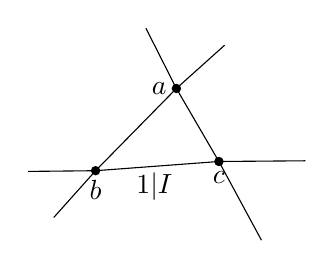
\begin{tikzpicture}[x=.009cm,y=-.009cm]
\draw (8,244)--(103,243)--(277,230)--(399,229); \draw (44,309)--(103,243)--(217,127)--(285,66); \draw (174,42)--(217,127)--(277,230)--(337,341);
\fill (217,127) circle (1.7pt) node[left] {$a$}; \fill (103,243) circle (1.7pt) node[below] {$b$};
\fill (277,230) circle (1.7pt) node[below] {$c$}; \node at (186,266) {$\unsure{1|I}$};
\end{tikzpicture}}

Supposons d'abord qu'on peut trouver
des droites $D_a,D_b,D_c$ passant par les
sommets $a,b,c$, qui ne soient pas concourantes.
On trouve une configuration,
associée canoniquement à l'ens
$J$ à trois éléments, avec comme
\inserted{9} sommets les $a_i$ $(i\in J)$ de
$K_J$, les intersections $\alpha_i$ $(i\in J)$
des $D_{a_i}$ avec $D_i$ (\uline{NB} $a_i$ est
le sommet de $K_J$ opposé à $D_i$)
\figure{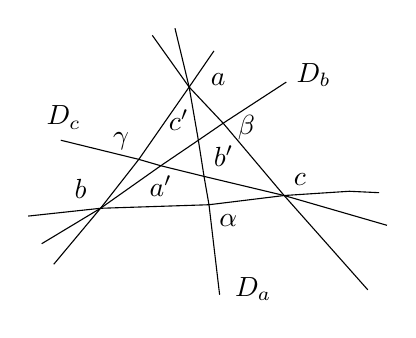
\begin{tikzpicture}[x=.009cm,y=-.009cm]
\draw (70,373)--(136,294)--(190,225)--(261,123)--(296,72);
\draw (209,50)--(261,123)--(309,174)--(395,276)--(513,409);
\draw (34,305)--(136,294)--(289,289)--(395,276)--(487,270)--(529,272);
\draw (241,40)--(261,123)--(274,198)--(282,249)--(289,289)--(304,416);
\draw (53,344)--(136,294)--(221,234)--(274,198)--(309,174)--(398,116);
\draw (80,198)--(190,225)--(221,234)--(282,249)--(395,276)--(540,318);
\node[right] at (278,113) {$a$}; \node[above left] at (130,294) {$b$};
\node[above right] at (395,276) {$c$}; \node[right] at (399,106) {$D_b$};
\node[above] at (84,196) {$D_c$}; \node[right] at (312,408) {$D_a$};
\node[below right] at (290,289) {$\alpha$}; \node[right] at (316,180) {$\beta$};
\node[above left] at (190,225) {$\gamma$}; \node[below] at (221,234) {$a'$};
\node[above right] at (282,249) {$b'$}; \node[above left] at (274,198) {$c'$};
\end{tikzpicture}}
les $a'_i$ $(i\in J)$ intersections de $D^{\unsure{\prime|1}}_{a_j}$ et $D_{a_{\deleted{\unsure{j}}k}}$ (où
$J=\{i,j,\unsure{h|k}\}$). \deleted{\unsure{L}} La figure montre comment
les sommets se répartissent suivant les 6
ps. droites $D_i,D_{a_i}$, et \deleted{la configuration est} \inserted{le $D_{J'}$ correspondant}
(avec les 6 ps. droites) est compl\textsuperscript{t} décrit,
quand on a décrit les structures polygônales
% archive sheet number: 51

\scanpage{53}
sur \deleted{\unsure{des}} \inserted{chacun} des \unsure{ens} des quatre sommets
$a_i,\alpha_i,a'_j,a'_k$ \unsure{se} trouvant sur un $D_{a_i}$,
i.e. en \unsure{précisant|disant} lequel, parmi les trois
sommets $\alpha_i,a'_j,a'_h$ distincts de $a_i$, est
\uline{opposé} à $a_i$. On voit que si la
figure \inserted{1-dimensionnelle} provient d'un arrang\textsuperscript{t} 2-dimensionnel,
alors il y a \inserted{(Cas I)} un ordre circulaire
% slanted
\margin{Il y a une autre possibilité, c'est que pour \deleted{\unsure{tout}} $i\in J$, $a_i$ soit opposé à $\alpha_i$ (cas II)}
sur $J$ (unique), tel que $a_i$ soit opposé,
sur $D_{a_i}$, à $a'_{i+1}$. (\uline{NB} Dans le cas
de figure choisi, cet ordre circulaire est
$\unsure{abc^{\circlearrowright}|abc^{\rightarrow}|abc}$).
\deleted{On \unsure{fera|verra|trouve}} \deleted{On voit que les configurations} \deleted{\unsure{Quand}}
\deleted{2-dimensionnelles} La situation $K$, donc
$K_{J'}$, \deleted{\unsure{prov}} et $K_J$, provient d'un arr. 2-dimensionnel,
alors, \deleted{\unsure{les}} désignant par
$\lambda_i$ $(i\in J)$ \deleted{les} \inserted{l'}arête de $K_J$ \deleted{qui con} portée
par $D_i$ qui contient $\alpha_i$, les $\lambda_i$ $(i\in J)$
font un syst. d'arêtes compatible avec
l'orientation dans le cas I, et non compatible
dans le cas II.

(A6) \deleted{L'orien} Dans le cas d'un système
de trois ps droites $J\in\unsure{\mathfrak P_3|\mathcal P_3}(I)$ non concourantes,
tel que \unsure{tt|toute} autre ps. droite passe par un des
trois sommets \inserted{$a_i$} de $K_J$, et lorsqu'on peut trouver
pour chaque $a_i$ une $d_{a_i}$ qui passe par $a_i$ et
% archive sheet number: 52

\scanpage{54}\mspage{12}
\deleted{distincte \unsure{des|de} \unsure{$\notin$|$\varnothing$|$\ell$}} $\in I\setminus J$, de façon que les trois
$D_{a_i}$ soient non concourantes, on exige
$(1^\circ)$ que l'\deleted{configuration}\inserted{arr.\ 1-dim} $K_{J'}$ de 6 droites obtenu
soit du cas (\deleted{\unsure{II}}I) ou (II) ci dessus, et
$(2^\circ)$ que l'orientation de $K_J$ défini par la
prescription précédente ne dépende pas du
choix de $J'$.

Il reste enfin à regarder le cas où
quel que soit le système $a_i$ $D_{a_i}$ ($D_{a_i}\in I\setminus J$
passant par $a_i$), celles-ci sont concourantes.
% slanted
\margin{\unsure{de plus au|de plus aucun} fait que $D_{j\in I\setminus J}$ \unsure{passe} par un des trois sommets}
Mais cela implique que \deleted{l'arrang\textsuperscript{t} est} $\operatorname{card} I=6$,
et que l'arrang\textsuperscript{t} est \inserted{isomorphe à} l'arrangement
\unsure{standart|standard} \deleted{de} formé de $7=4+3$ sommets
et 6 ps. droites (qui sont des triangles),
\figure{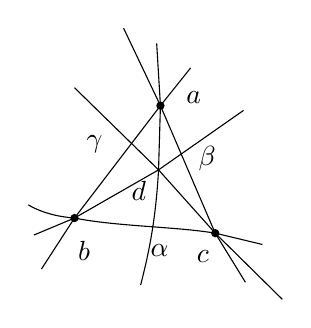
\begin{tikzpicture}[x=.012cm,y=-.012cm]
\draw (29,293)--(64,239)--(155,120)--(187,80);
\draw (116,38)--(155,120)--(213,255)--(245,307);
\draw (151,54)--(155,120)--(153,188).. controls (150,241) and (143,275)..(134,310);
\draw (64,101)--(153,188)--(213,255)--(284,325);
\draw (15,225).. controls (32,235) and (51,238)..(64,239).. controls (109,248) and (171,248)..(213,255)--(263,267);
\draw (21,257)--(64,239)--(153,188)--(243,125);
\fill (155,120) circle (1.5pt); \fill (64,239) circle (1.5pt); \fill (213,255) circle (1.5pt);
\node[right] at (172,111) {$a$}; \node[below] at (74,253) {$b$}; \node[below] at (200,263) {$c$};
\node[below left] at (150,190) {$d$}; \node[below] at (154,257) {$\alpha$};
\node[right] at (185,176) {$\beta$}; \node[left] at (104,161) {$\gamma$};
\end{tikzpicture}}
avec quatre sommets triples, les six ps.
droites étant les ps. droites qui les relient
deux à deux, les trois points d'intersection
supplémentaires étant les intersection des
paires de ps. droites ``opposées''. La situation
combinatoire 1-dimensionnelle (ne comport\textsuperscript{t}
que des triangles) est entièr\textsuperscript{t} décrite
par l'ens des quatre sommets triples.
La situation 2-dimensionnelle correspondante
est aussi \unsure{standart|standard} ($=$ groupe d'autom $\unsure{\mathfrak S|\mathscr S}_4$)
On trouvera la description suivante :
% archive sheet number: 53
